\documentclass[conference]{IEEEtran}



\usepackage[spanish,USenglish]{babel} % español, ingles
\usepackage[utf8]{inputenc} % acentos sin codigo

\usepackage{float} % acentos sin codigo
\usepackage{hyperref}

%\usepackage{graphicx}
\usepackage{subcaption}




\ifCLASSINFOpdf
   \usepackage[pdftex]{graphicx}
  % declare the path(s) where your graphic files are
   \graphicspath{{./figuras/}}
  % and their extensions so you won't have to specify these with
  % every instance of \includegraphics
   \DeclareGraphicsExtensions{.pdf,.jpeg,.png,.jpg}
\else
 
\fi


\hyphenation{op-tical net-works semi-conduc-tor}


\begin{document}
\selectlanguage{spanish}
\title{Optimización de operadores PDI con CUDA}

\author{\IEEEauthorblockN{\textbf{Alvaro Camacho Mora}}
\IEEEauthorblockA{Escuela de Ingenier\'ia en Electr\'onica\\
Instituto Tecnol\'ogico de Costa Rica\\
Procesamiento Digital de Imágenes\\
IIIC-2018}}


\maketitle
\thispagestyle{plain}
\pagestyle{plain}

\begin{abstract}
Se aborda la optimización del algoritmo de aplicar el filtro de máximos a imágenes de diferentes tamaños utilizando un GPU. El problema es atacado utilizando diferentes técnicas de optimización, empezando con un algoritmo sencillo para después utilizar técnicas como kernel separable, kernel separable mas procesamiento multi-hilo y finalizando con kernel separable mas procesamiento multi-hilo con memoria compartida (\textit{shared memory}). El resultado de cada kernel optimizado es comparado con una implementación trivial ejecutada en CPU.

\end{abstract}


\section{\textbf{Introducción}}
Este documento trata sobre la optimización del tiempo de ejecución del  algoritmo de filtro de máximos utilizando técnicas de paralelización orientada a procesadores gráficos (GPU). Se dará una visión general de la arquitectura de un GPU y el paradigma de programación de las técnicas utilizadas para la optimización y así explicar el porque de la reducción en el tiempo de ejecución del algoritmo.\\
Se tendrá como base para determinar la diferencia en los resultados el algoritmo ejecutado en el procesador general (CPU) y se comparara con los resultados utilizando la técnica \textit{L2-norm}.

\section{\textbf{Filtro de Máximos}}
El filtro máximos se considera un filtro estadístico de orden ya que funcionan ordenando los valores de la vecindad del punto de interés. Como su nombre lo dice dado una ventana (kernel) se escogerá el valor máximo entre la vecindad del punto de interés, que sera el centro del kernel.\\
El resultado que se obtendrá al someter una imagen a un filtro de máximo sera la eliminación de del ruido de pimienta o píxeles negros. Dado su funcionamiento, tiene como principal desventaja es que produce un aclaramiento de la imagen debido a que los elementos negros son eliminados o dicho de otra manera se ensanchan las zonas claras y adelgazan las zonas oscuras \cite{max}. La figura \ref{maxF} muestra como se adelgazan esas zonas negras en la imagen original cuando se compara con la imagen filtrada.

\begin{figure}[H]
\centering

\includegraphics[width=4cm]{maxF}
\caption{Efecto del filtro de máximos}
\label{maxF}
\end{figure}

\section{\textbf{GPU}}
En días recientes los GPU se han vuelto muy populares para migrar algoritmos de gran complejidad y que pueden aprovechar el poder de procesamiento de los GPU para acelerar el proceso de ejecución. Dos de las ventajas principales por las que se esta tendiendo al uso de GPU para procesamiento paralelo es la arquitectura en si del GPU que provee grandes cantidades de recurso y además una plataforma para el desarrollo de aplicaciones orientadas a GPU como lo es CUDA. En esta sección se brindaran detalles sobre estos dos elementos.
\subsection{\textbf{Arquitectura}}
Los CPU modernos son sistemas integrados de alto poder de procesamiento, pero mucho de su poder se reduce en el uso de muchos de sus transistores en la memoria cache y el control flujo del programa, esto debido a que como son procesadores de uso general deben enfrentar diferentes problemas y tienen que tener la capacidad de responder ante diferentes necesidades. Por otra parte un GPU, ejecuta el mismo programa en sus diferentes elementos de procesamiento y con esto se reduce dramáticamente el uso de sofisticados diseños de control de flujo. Por otro lado las aplicaciones que son enviadas a un GPU son orientadas a tener gran cantidad de procesamiento aritmético por lo que se prioriza el poder de procesamiento sobre la cantidad de memoria cache\cite{info_cuda}.\\

La figura \ref{cpu_vs_gpu} muestra una comparación de un CPU con 4 núcleos con una arquitectura de un GPU. Claramente se puede ver como este CPU tiene la capacidad de ejecutar solamente 4 hilos en paralelo versus el GPU que tiene la capacidad de ejecutar muchos mas hilos en paralelo.

\begin{figure}[H]
\centering
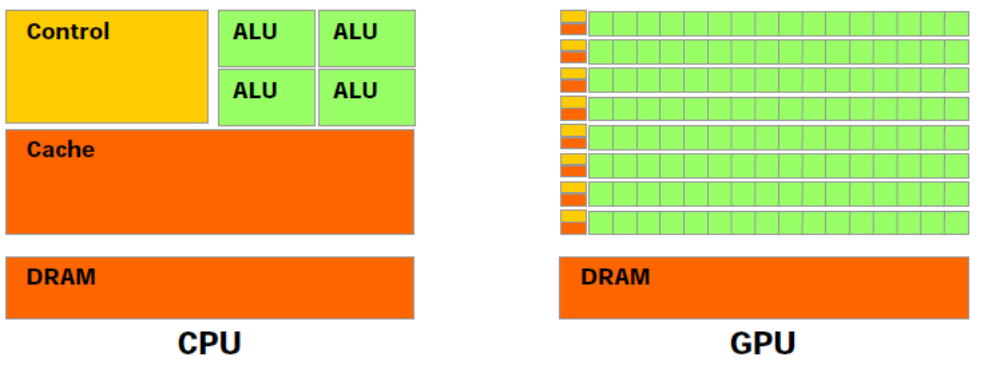
\includegraphics[width=8cm]{cpu_vs_gpu}
\caption{Comparación de arquitecturas entre un CPU y GPU \cite{cuda_by_example}}
\label{cpu_vs_gpu}
\end{figure}

Una arquitectura clásica de un GPU es mostrada en la figura \ref{gpu}, donde se puede ver que se tiene una cantidad de multiprocesadores que a su vez tienen diferentes unidades funcionales. Cabe mencionar que, además cada multiprocesador tiene diferentes opciones de memoria como lo son: 
\begin{list}{--}{}
\item
\textit{Shared Memory}: 49 kB
\item
\textit{Texture cache}: 64 kB
\item
\textit{Constant cache}: 64 kB
\item
\textit{Registros}: 65536
\item
\textit{Memoria global}: 2 GB
\end{list}

Se debe mencionar que estos numero son para el GPU utilizado en esta implementación (GeForce 960M) y que la memoria global si puede ser compartida entre los diferentes multiprocesadores. Esta arquitectura usa una arquitectura SIMT (\textit{Single Instruction Multiple Thread}), lo que indica que cada cada instrucción simple es ejecutada en paralelo por múltiples hilos.\\

Un detalle que se debe tomar en cuenta es que solamente a través de memoria global se puede dar una pseudo comunicación entre multiprocesadores, por lo que esto se debe tomar en cuenta pues las lecturas/escrituras son muy costosas.


\begin{figure}[H]
\centering
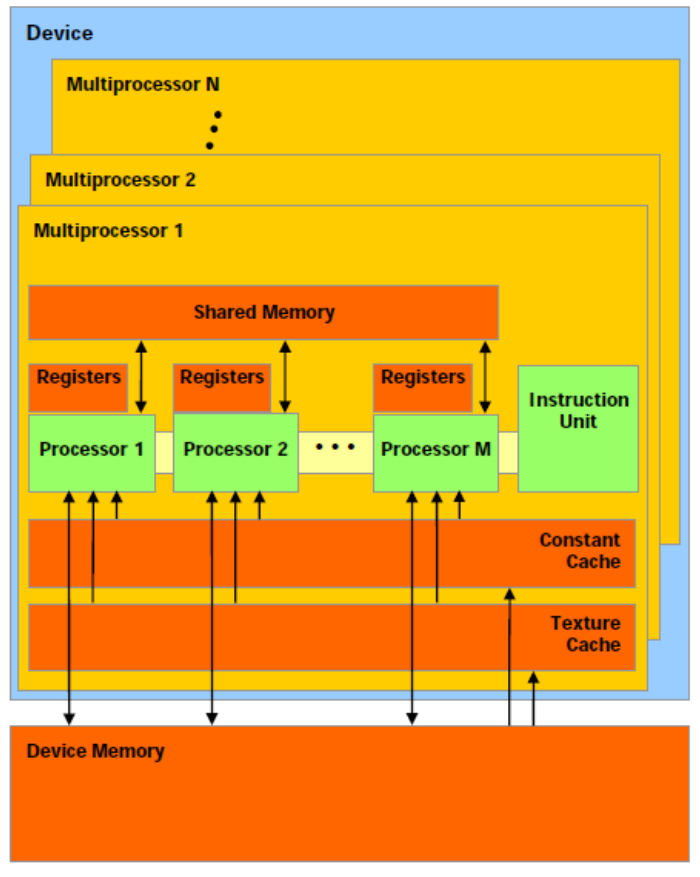
\includegraphics[width=6cm]{gpu}
\caption{Arquitectura clásica de un GPU\cite{victor_cuda}}
\label{gpu}
\end{figure}

\subsection{\textbf{CUDA: Modelo de Programación}}
El modelo de programación utilizado en CUDA trata de aplicar el lema ''divide y vencerás''  ya que al no tener algún tipo de memoria que logre la comunicación entre multiprocesadores se debe dividir el problema en pedazos mas simples para poder ejecutar la aplicación eficientemente.\\

La figura \ref{cuda_model} muestra una cuadricula (grid) dividida en bloques que a su vez estos bloques contienen hilos. El bloque es ejecutado en un multiprocesador especifico, por lo que cada uno de los hilos dentro de este bloque podrá comunicarse entre ellos pero no se podrá comunicar con otro bloque. Asimismo cada bloque tendrá un único identificador 2D dentro de la cuadrilla y probablemente cada hilo un identificador 3D dentro de cada bloque.\\

Otro importante concepto que se debe tener en cuenta es el de \textit{warp} que básicamente se puede definir como un bloque de 32 threads agrupados consecutivamente que puede correr una misma instrucción y puede comunicarse entre ellos \cite{warp_cuda}.

\begin{figure}[H]
\centering
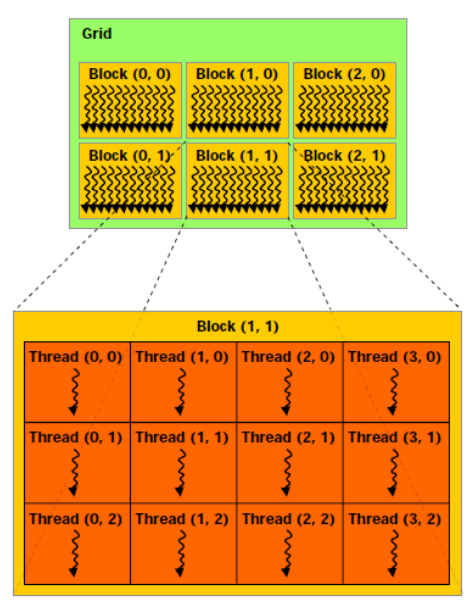
\includegraphics[width=6cm]{cuda_model}
\caption{Modelo de programacion de CUDA \cite{cuda_by_example}}
\label{cuda_model}
\end{figure}

\section{\textbf{Metodología}}
En esta sección se explica la metodología seguida para lograr los resultados que se explicaran en la siguiente sección.
\subsection{\textbf{Sistema utilizado}}
La tabla \ref{table_hrdware_software} muestra los detalles sobre el hardware/software utilizado para correr cada uno de las optimizaciones que se plantearan mas adelante:
\begin{table}[h]
\caption{Características de software y hardware utilizadas} % title name of the table
\centering % centering table
\begin{tabular}{l c c rrrrrrr} % creating 10 columns
\hline\hline % inserting double-line
 Dispositivo/Software & Modelo/Versión/Valor\\ [0.5ex]
\hline % inserts single-line
CPU & Intel Core i7-6700HQ\\[0.5ex]
CPU DRAM & 12GB\\[0.5ex]
GPU & NVIDIA GeForce GTX 960M\\[0.5ex]
Lti::lib & 2\\ [0.5ex]% Entering row contents
CUDA Toolkit & 10.0\\[0.5ex]
Cmake & 3.10.2\\[0.5ex]
Ubuntu & 18.0.4 \\[0.5ex]
\hline % inserts single-line
\end{tabular}
\label{table_hrdware_software}
\end{table}

\subsection{\textbf{Pasos de Optimización}}
En esta sección se detallan los diferentes pasos y optimizaciones hechas en cada uno de ellas para reducir el tiempo de ejecución. También se detallan implementaciones del kernel ejecutadas en el CPU pues estas son necesarias como parámetros de referencia.
\subsubsection{\textbf{Función lti::maximumFilter}}
Como parte de los objetivos del proyecto se debió ejecutar una función parcialmente optimizada como las que son parte de bibliotecas como lo es LTI-lib-2. La función escogida fue: lti::maximumFilter.\\
Esta función es una implementación muy sencilla de conseguir ya que únicamente se necesita como entrada al constructor el tamaño del kernel y después hacer uso del método \textit{apply} para obtener un imagen filtrada\cite{lti_max}.
\subsubsection{\textbf{Kernel Trivial GPU}}
Como parte del instructivo se proveyó de un algoritmo sencillo para aplicar el filtro de máximos a una imagen. Este código debió ser ejecutado como punto de partida para las optimizaciones realizadas a nivel de GPU.
\subsubsection{\textbf{Kernel Trivial CPU}}
Básicamente este es el mismo algoritmo sin ninguna optimización entregado como parte del enunciado del proyecto, pero fue ligeramente modificado para que fuese ejecutado en el CPU en lugar del GPU. Esto fue realizado para tener un punto de comparación tanto a nivel de resultados como de tiempo de ejecución.
\subsubsection{\textbf{Kernel Separable}}
Los filtros separables es de las tecnicas de optimizacion basicas mas poderozas que se tienen ya que como es descrito en \cite{victor_cuda}\cite{separable_pablo} pues se pasa de n*m operaciones para obtener cada píxel(donde n es la cantidad de filas y m la cantidad de columnas del kernel). Esta propiedad de separabilidad transforma el kernel 2D en dos kernel sencillos 1D que reduce la cantidad de operaciones por cada píxel a n+m.
\subsubsection{\textbf{Kernel Separable + Multi-Threading}}
Las dos implementaciones anteriores a nivel de GPU fueron ejecutadas utilizando únicamente 1 Thread y 1 block. Esto es como si se estuviese ejecutando en un CPU muy básico. Ahora bien, con la utilización de múltiples bloques e hilos se aumenta el poder de procesamiento.
Los principales cambios que se dieron en el kernel es la eliminación de los ciclos \textit{for} que realizaban el recorrido de la imagen píxel por píxel. Esto es gracias a que con esta nueva implementación cada uno de los threads va a ser el encargado de manejar un píxel en la imagen.\\
La figura \ref{threads_blocks} muestra por ejemplo una imagen de 5x5 donde la imagen va a ser cargada en el grid y cada thread va a manejar un pixel. Otro detalle a mencionar es lo que se explica en \cite{cuda_by_example}, donde se recomienda realizar la asignación del numero de threads y bloques de una forma que la cantidad de bloques sea múltiplo de la cantidad de threads escogida para aumentar la eficiencia y que cada warp sea intensivamente utilizado.
\begin{figure}[H]
\centering
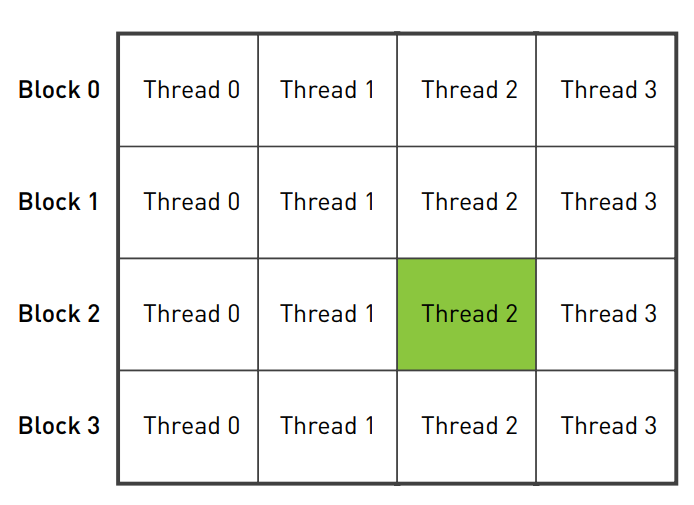
\includegraphics[width=5cm]{threads_blocks}
\caption{Representación del acomodo de los threads y blocks dentro del GPU para una imagen de 5x5 \cite{cuda_by_example}}
\label{threads_blocks}
\end{figure}

\subsubsection{\textbf{Kernel Separable + Multi-Threading + Shared Memory}}
Esta etapa de optimización se va a utilizar teniendo en cuenta las etapas anteriores mas una nueva técnica de optimización llamada \textit{shared memory}. Esta técnica utiliza una memoria que esta alojada en cada uno de los bloques y el acceso a ella por cada uno de los threads es mucho menor que lo que tomaría realizar lecturas a memoria global.\\
Dado que se esta hablando de una memoria dentro de cada bloque, se debe copiar la sección de la imagen que se quiere procesar desde memoria global a la memoria compartida. Este es un paso que se debe realizar pero el \textit{overhead }creado es compensado con la velocidad de procesamiento que se logra utilizando esta memoria. Posterior a que se dio la copia el procesamiento es muy similar al que se ha seguido hasta el momento donde cada thread del bloque lee la memoria compartida, procesa el píxel y se guarda en memoria global como resultado del procesamiento.\\
Una parte extra que se debe tomar en cuenta es que debido a que se esta copiando una parte de la imagen, cuando se copia a memoria compartido, en los bordes van a haber problemas pues no se tienen los píxeles de la imagen original. La figura \ref{shared_mem} muestra este concepto y aunque la representación no corresponde a un kernel separable, el concepto es el mismo . Con esto se estarían ''desperdiciando'' algunos threads, sin embargo la ganancia vale la pena \cite{cuda_by_example}\cite{victor_cuda}\cite{nvidia_separable}.
\begin{figure}[H]
\centering
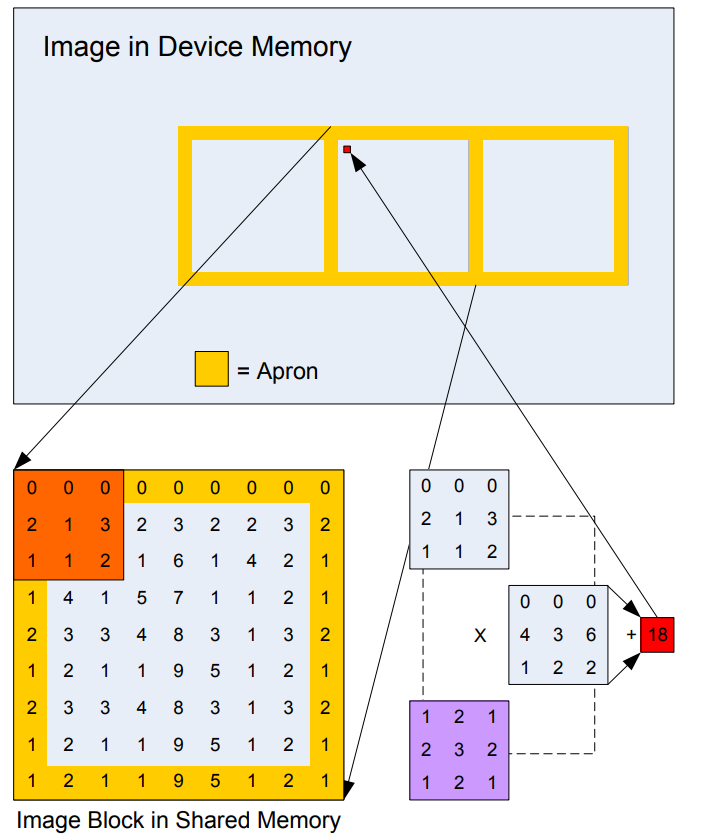
\includegraphics[width=5cm]{shared_mem}
\caption{Representación de la copia de datos de memoria principal a memoria compartida \cite{victor_cuda}}
\label{shared_mem}
\end{figure}

\subsection{\textbf{Detección de diferencias en la imagen de salida}}
Para evaluar si las imagenes de salida de cada uno de los kernels es igual al resultado base (CPU y GPU) se va a utilizar la norma Euclidiana o L2-nomr que es una evaluacion matematica para estimar la diferencia entre dos vectores. Bajo este supuesto, si el resultado de evaluar la imagen de referencia contra la salida de cada kernel es igual a cero las imagenes son iguales pues la difenrencia entre ambos vecotres es cero. En caso que se de un valor diferente a cero se estaria en presencia de de algun error en el algoritmo \cite{log0}\cite{norm2}.


\subsection{\textbf{Medición del tiempo de ejecución}}
Para evaluar el tiempo que tomo el tiempo la ejecución de cada algoritmo se siguieron dos enfoques:
\begin{list}{•}{}
\item
CPU: se utilizaron los métodos dentro de la biblioteca \textit{chrono} para realizar la medición del tiempo para los kernel ejecutados en el CPU.
\item
GPU: para el caso de los kernel ejecutados en el GPU se utilizaron los métodos pertenecientes a la clase \textit{cudaEvent\_t}. También fue utilizada la aplicación \textit{nvprof} que es parte del toolkit de CUDA, pero únicamente fue utilizada para comprobar el método de cudaEvent\_t.
\end{list}

Para ser mas objetivos en la obtención de resultados reales, se ejecuto 30 veces cada kernel y se tomo el tiempo promedio para el reporte de los resultados. Además se evaluó la varianza del tiempo de ejecución cuando se utilizo imágenes de diferente tamaño.

\section{\textbf{Resultados}}
\subsection{\textbf{Reducción de Tiempos de Ejecución}}
Uno de los principales objetivos de este proyecto es la evaluación de la reducción del tiempo de ejecución al aplicar los diferentes kernels optimizados. La tabla \ref{table_optimizacion_tiempo} muestra los tiempos de ejecución promedios para cada kernel en donde se puede observar como los kernel ejecutados en el CPU sin muy rápidos, incluso mas rápidos que la ejecución en el GPU utilizando memoria compartida. Claramente se ve una tendencia a que cada kernel optimizado en el GPU reduce significativamente el tiempo de ejecución como se puede observar en la figura \ref{time_vs_opt} como cada optimización hace que baje abruptamente la curva. Cabe mencionar que que el eje vertical de la figura \ref{time_vs_opt} ha sido cambiado a una escala logarítmica para poder observar fácilmente las tendencias de los datos.\\


\begin{table}[h]
\caption{Tiempos promedio de ejecución para cada kernel} % title name of the table
\centering % centering table
\begin{tabular}{l c c rrrrrrr} % creating 10 columns
\hline\hline % inserting double-line
Kernel & Tiempo de Ejecución (ms)\\ [0.5ex]
\hline % inserts single-line
LTI:lib & 0.01078\\[0.5ex]
Trivial CPU & 0.06409\\[0.5ex]
Trivial GPU & 909.400\\[0.5ex]
Separable & 414.465\\ [0.5ex]% Entering row contents
Separable + MTH & 0.11727\\[0.5ex]
Separable + MTH + Shared Memory & 0.07793\\[0.5ex]
\hline % inserts single-line
\end{tabular}
\label{table_optimizacion_tiempo}
\end{table}

\begin{figure}[H]
\centering
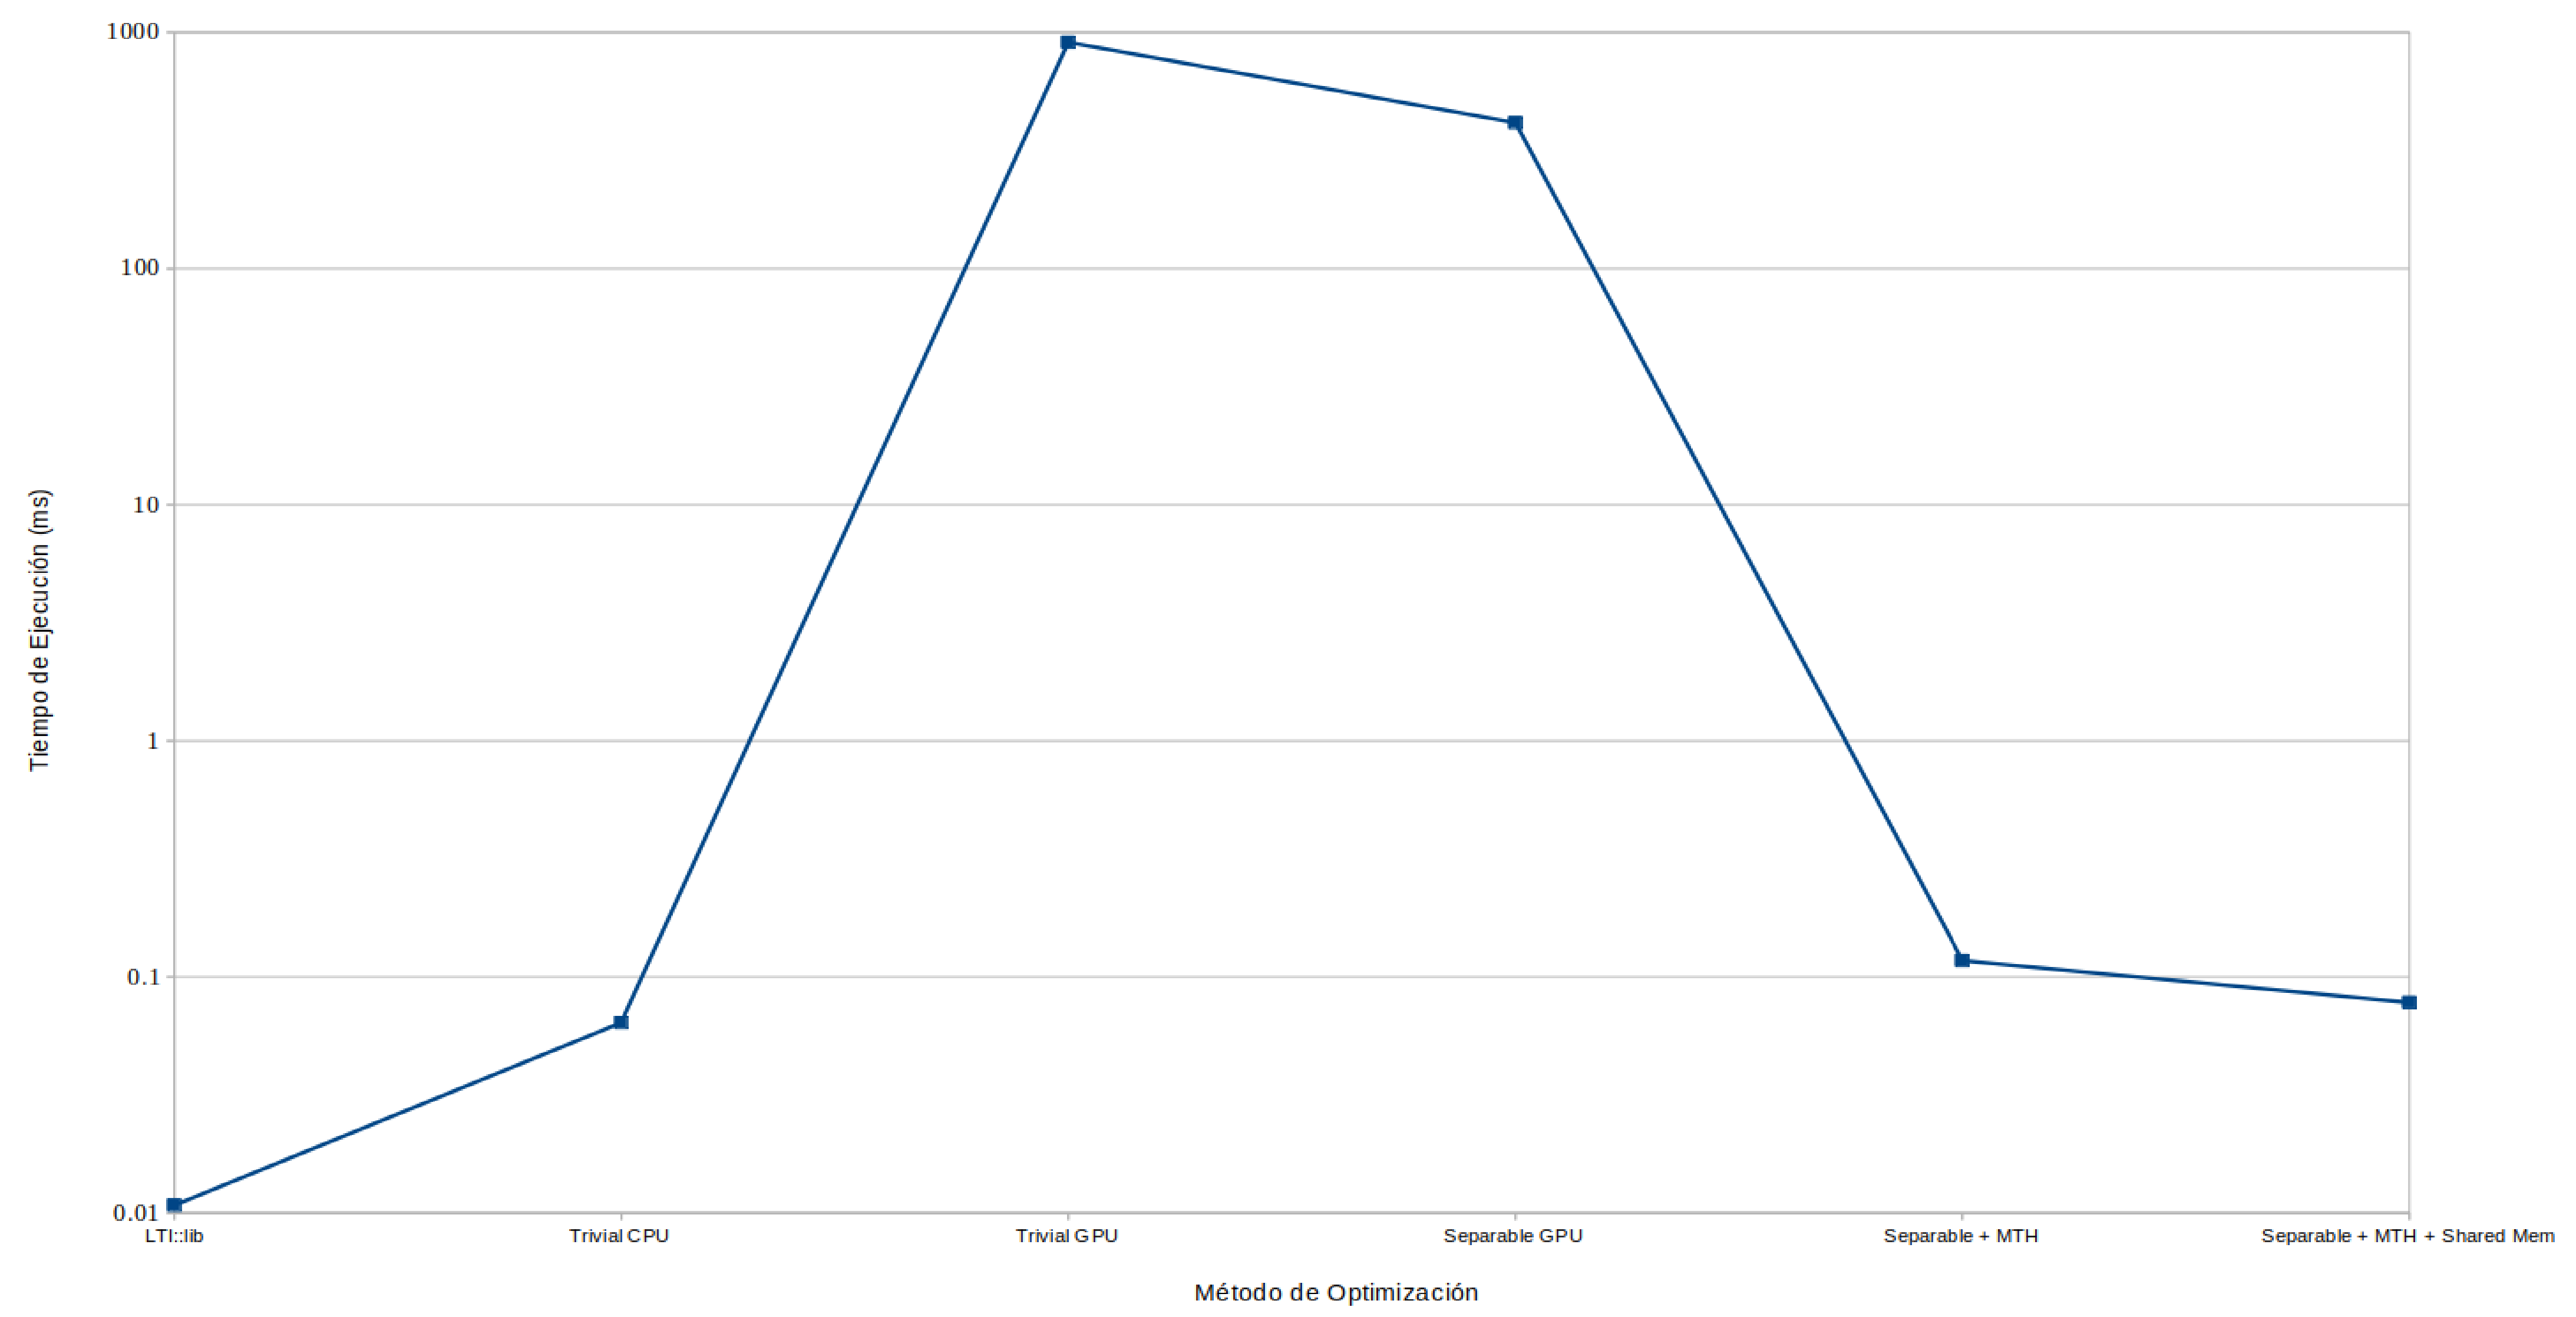
\includegraphics[width=9cm]{time_vs_opt}
\caption{Tiempo de ejecución versus algoritmo utilizado}
\label{time_vs_opt}
\end{figure}

Cabe mencionar como detalle adicional que para esta evaluación se utilizo la imagen de la figura \ref{lenna} la cual tiene un tamaño de 720x430. 

\begin{figure}[H]
\centering
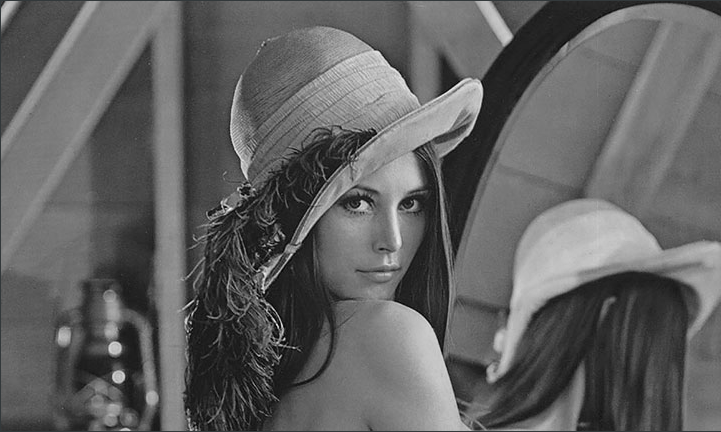
\includegraphics[width=6cm]{lenna}
\caption{Imagen utilizada para la evaluación del tiempo de ejecución de cada kernel.}
\label{lenna}
\end{figure}

\subsection{\textbf{Tiempos de ejecución con respecto al tamaño de la imagen}}
El objetivo con esta evaluación es saber cuando tiempo le toma a cada kernel en promedio ejecutar el filtrado cuando el tamaño de la imagen aumenta. Para esto se evaluaron 5 imágenes con tamaños estándares y los resultados se pueden ver en la tabla \ref{table_optimizacion_resol}. Además en la figura \ref{resol} se puede observar la tendencia de cada kernel, cabe mencionar que el eje vertical esta en escala logarítmica para que las diferentes tendencias puedan ser observables.\\

Como era de esperar, se observa como cada kernel aumenta su tiempo de ejecución cuando el tamaño de la imagen aumenta. Otro aspecto a destacar es que las implementaciones en el CPU son las que mas rápido ejecutan el filtrado.

\begin{table}[h]
\caption{Tiempos promedio de ejecución para cada kernel tomando en cuenta imágenes de diferente tamaño} % title name of the table
\centering % centering table
\begin{tabular}{l c c rrrrrrr} % creating 10 columns
\hline\hline % inserting double-line
Kernal & 320x240 & 420x240 & 620x480 & 800x600 & 1280x720\\ [0.5ex]
\hline % inserts single-line
LTI:lib & 0.00244&	0.00361 &	0.01012 &	0.01472&	0.03543\\[0.5ex]
Trivial CPU & 0.01578	&0.02106&	0.06592&	0.10515	&0.19727\\[0.5ex]
Trivial GPU & 225.667	&296.032	&873.970&	1410.422&	2708.779\\[0.5ex]
Separable & 108.056	&141.907&	419.167&	675.951	&1298.293\\ [0.5ex]
Separable + MTH & 0.03530&	0.05136&0.10963&	0.16019	&0.29822\\[0.5ex]
Sep+MTH+Sh Mem & 0.02634	&0.03925	&0.07764&	0.11203&0.20696\\[0.5ex]
\hline % inserts single-line
\end{tabular}
\label{table_optimizacion_resol}
\end{table}

\begin{figure}[H]
\centering
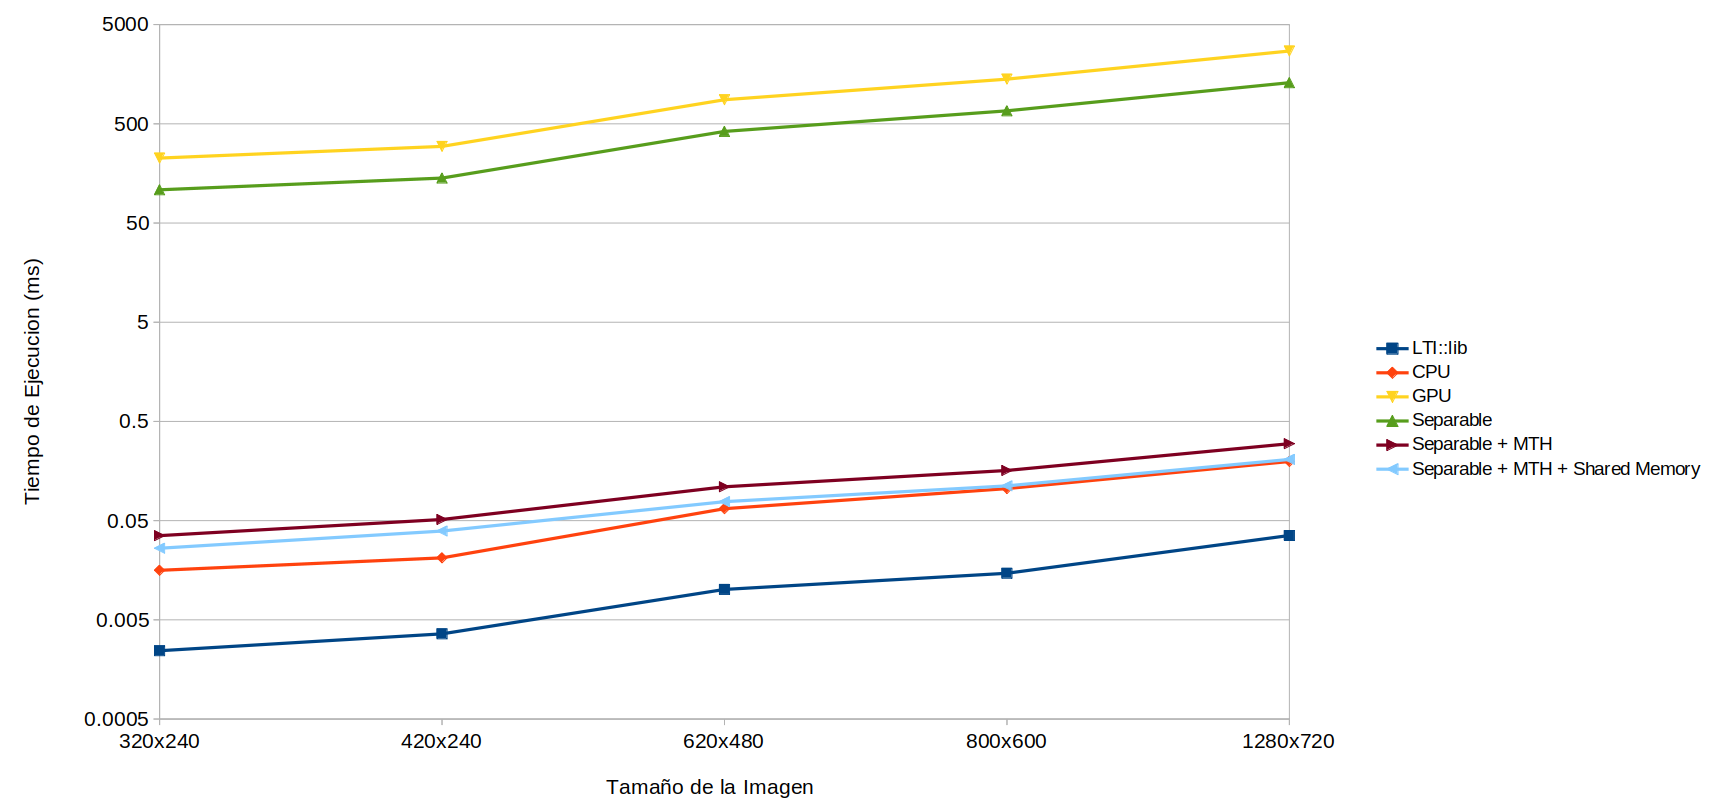
\includegraphics[width=9.5cm]{varianza}
\caption{Tendencia del tiempo de ejecución cuando se aumenta el tamaño de la imagen}
\label{resol}
\end{figure}


\subsection{\textbf{Similitud de las imágenes de salida}}
Como se explico en la sección de metodología para la evaluación de las diferencias no solamente se aplico el factor visual si no que también se aplico un efecto matemático para evaluar que tan diferentes eran las imágenes con respecto a su referencia. El método que ha sido seleccionado es el llamado \textit{L2-norm} que se encarga de evaluar la diferencia entre dos vectores y cuyos resultados se resumen en la tabla \ref{table_l2norm}. En dicha tabla se puede observar como el resultado de aplicar el L2-norm es cero cuando se analiza la diferencia entre el kernel trivial, GPU trivial y separable. Las diferencias empiezan a mostrarse en el Separable + MTH y Separable + MTH + Shared Memory. 
\begin{table}[h]
\caption{Difencias promedio entre imagen resultado y la referencia (Kernel CPU)} % title name of the table
\centering % centering table
\begin{tabular}{l c c rrrrrrr} % creating 10 columns
\hline\hline % inserting double-line
Kernel & Tiempo de Ejecución (ms)\\ [0.5ex]
\hline % inserts single-line
Lti::lib & 7.2$ e^{-2}$\\[0.5ex]
GPU & 0\\[0.5ex]
Separable & 0\\[0.5ex]
Separable + MTH & 5.523$ e^{-3} $\\ [0.5ex]% Entering row contents
Separable + MTH + Shared Memory & 1.336$ e^{-1}$\\[0.5ex]
\hline % inserts single-line
\end{tabular}
\label{table_l2norm}
\end{table}

La figura \ref{img_results} muestra el resultado de pasar la figura original de Lenna de la figura \ref{lenna} por cada uno de los kernels. Cabe destacar que en general son bastante parecido, únicamente el kernel con shared memory produce resultados con desviación mas grande, aunque presenta una similitud razonable con el kernel LTI::lib

\begin{figure}[H]
  \begin{subfigure}[b]{0.2\textwidth}
    \centering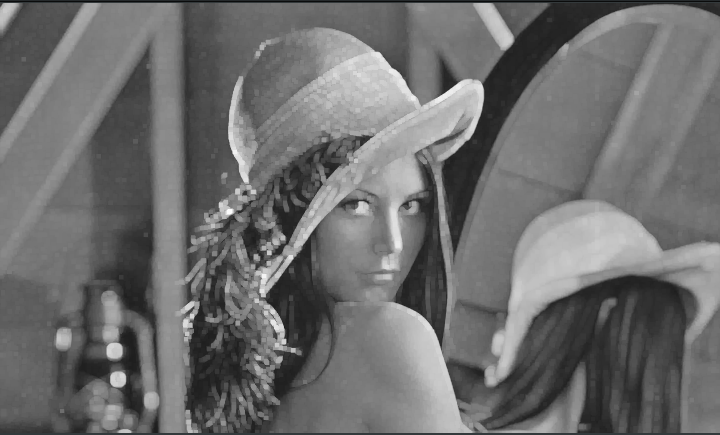
\includegraphics[width=3.5cm]{lenna_gpu}
    \caption{Lenna con kernel Trivial GPU}
  \end{subfigure}
  \begin{subfigure}[b]{0.2\textwidth}
    \centering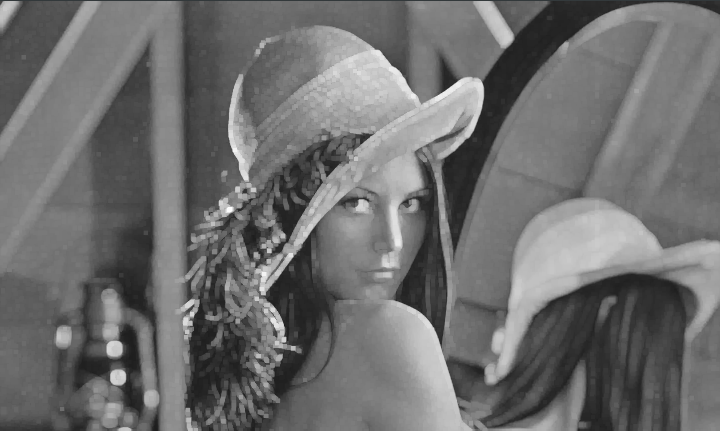
\includegraphics[width=3.5cm]{lenna_cpu}
    \caption{Lenna con kernel Trivial CPU}
  \end{subfigure}
 
  \begin{subfigure}[b]{0.2\textwidth}
    \centering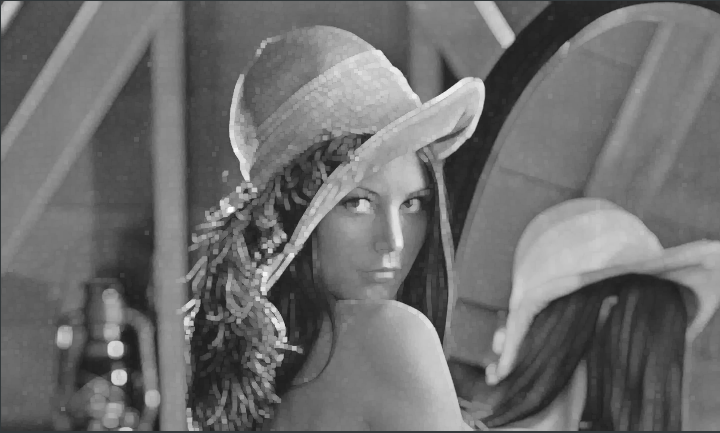
\includegraphics[width=3.5cm]{lenna_separable}
    \caption{Lenna con kernel Separable}
  \end{subfigure}
  \begin{subfigure}[b]{0.2\textwidth}
    \centering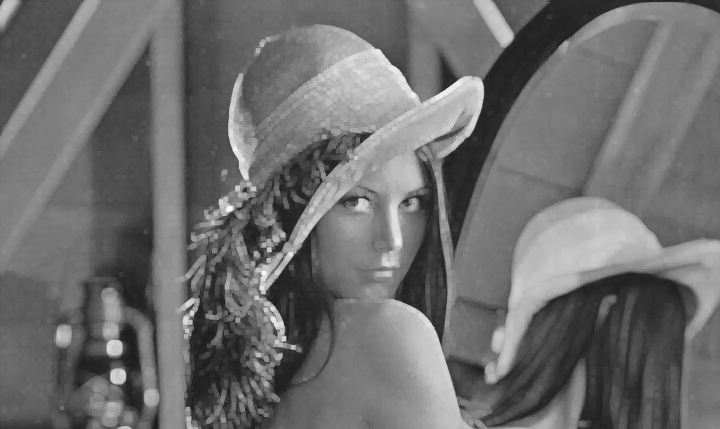
\includegraphics[width=3.5cm]{lenna_mth}
    \caption{Lenna con kernel Separable + MTH}
  \end{subfigure}
  
  \begin{subfigure}[b]{0.2\textwidth}
    \centering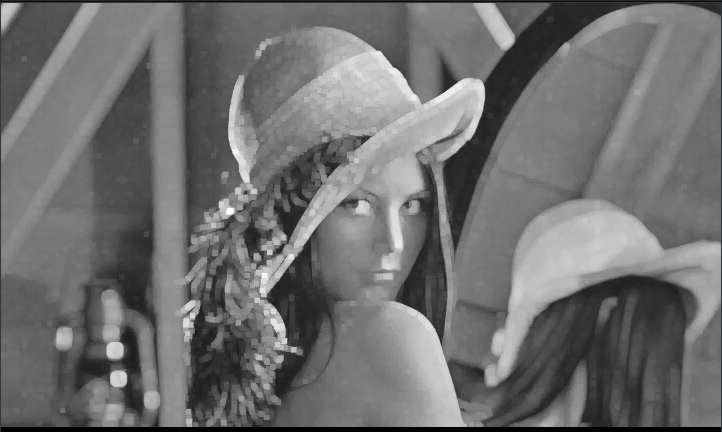
\includegraphics[width=3.5cm]{lenna_shared}
    \caption{Lenna con kernel Separable + MTH + Shared Memory}
  \end{subfigure}
  \begin{subfigure}[b]{0.2\textwidth}
    \centering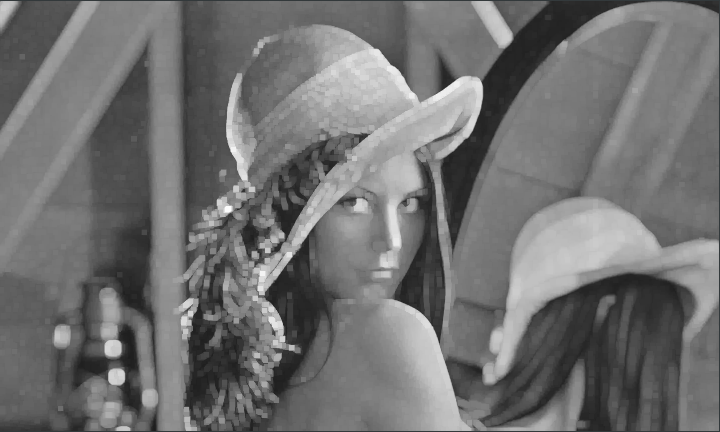
\includegraphics[width=3.5cm]{lenna_lti}
    \caption{Lenna con kernel LTI::lib}
  \end{subfigure}
  \caption{Imágenes resultado para cada kernel}
  \label{img_results}
\end{figure}


\section{\textbf{Conclusiones}}
Dados los resultados obtenidos la utilización del GPU para realizar tareas paralelas es una gran idea mas y cuando no se tiene un CPU poderoso que pueda hacer el trabajo. Además una implementación paralela en CPU necesita mucha infraestructura adyacente para poder correrse en diferentes hilos sin tener problemas,mientras que un GPU ofrece la infraestructura para correr aplicaciones paralelas en el hardware mismo. Esto reduciría enormemente el tiempo de desarrollo de aplicaciones reales que deben cumplir con apretados calendarios de desarrollo.\\
Es notable como agregar complejidad en el trabajo de paralelización disminuye el tiempo de ejecución, por ejemplo cuando se compara la implementación trivial con la implementación con el kernel separable + MTH + Shared memory donde se redujo el tiempo de ejecución cerca de 111670 veces.\\
La ganancia en cuanto a reducción de tiempo de ejecución también es notoria cuando se aumenta el tamaño de la imagen pues se obtuvieron resultados cercanos a los que se obtuvo con la ejecución del kernel en el CPU.\\
El resultado de las imágenes al ser comparadas con el kernel base indican que bajo un margen de tolerancia los resultados son bastante aceptables cuando se lleva al máximo nivel de optimización alcanzado en este trabajo que fue utilizando memoria compartida. Hacer as pruebas podrían ayudar a indicar donde esta el error en el resultado.
 
\section{\textbf{Áreas de Mejora/Trabajos futuros}}
\begin{list}{•}{}
\item
Implementar Shuffle Instructions: Las intrucciones suffle son instrucciones especializadas que permiten a los threads intereactuar entre ellos sin necesidad de ir a memoria compartida, es decir es una intereaccion que se realiza a nivel de registros \cite{warp_cuda}\cite{warp2}. Por lo que la implementación en procesamiento de imágenes es una herramienta poderosa para reducir aun mas el tiempo de ejecución.
\item
Evaluar como mejorar el resultados de los kernels: evaluar por que los resultados de las imágenes cuando se utiliza multithreading esta dando diferente a la referencia. Una posible hipótesis es que hayan algunos problemas en el direccionamiento de algunos threads/bloques. 
\end{list}


\bibliographystyle{IEEEtran}
\bibliography{bibliografia}

%


% that's all folks
\end{document}





